\documentclass[11pt,a4paper]{article}

% --- Paquetes compatibles con pdfLaTeX (estándar de Overleaf) ---
\usepackage[utf8]{inputenc}
\usepackage[T1]{fontenc}
\usepackage{lmodern}
\usepackage[spanish,es-tabla]{babel}
\usepackage[margin=2.5cm]{geometry}
\usepackage{xcolor}
\usepackage{graphicx}
\usepackage{tabularx}
\usepackage{booktabs}
\usepackage{longtable}
\usepackage{array}
\usepackage{enumitem}
\usepackage{fancyhdr}
\usepackage{titlesec}
\usepackage[hidelinks]{hyperref}

\graphicspath{{figuras/}}

% --- Páginas de flotantes alineadas arriba (no centradas verticalmente) ---
\makeatletter
\setlength{\@fptop}{0pt}
\setlength{\@fpsep}{1.5\baselineskip}
\makeatother

% --- Colores corporativos ULPGC ---
\definecolor{ulpgcblue}{RGB}{0, 102, 161}
\definecolor{ulpgcorange}{RGB}{243, 146, 0}

% --- Formato de títulos ---
\titleformat{\section}
  {\normalfont\Large\bfseries\color{ulpgcblue}}{\thesection}{1em}{}
\titleformat{\subsection}
  {\normalfont\large\bfseries\color{ulpgcblue!85!black}}{\thesubsection}{1em}{}
\titleformat{\subsubsection}
  {\normalfont\normalsize\bfseries\color{black!80}}{\thesubsubsection}{1em}{}

% --- Encabezado y pie de página ---
\pagestyle{fancy}
\fancyhf{}
\setlength{\headheight}{14pt}
\fancyhead[L]{\footnotesize\textcolor{gray}{ULPGC -- EII | Programación de Aplicaciones Móviles Nativas}}
\fancyhead[R]{\footnotesize\textcolor{gray}{Trabajo Final PAMN}}
\fancyfoot[C]{\thepage}
\renewcommand{\headrulewidth}{0.4pt}

% --- Configuración de tablas ---
\renewcommand{\arraystretch}{1.35}
\newcolumntype{L}[1]{>{\raggedright\arraybackslash}p{#1}}
\newcolumntype{Y}{>{\raggedright\arraybackslash}X}

% --- Marca para los datos que solo pueden completarse más adelante ---
\newcommand{\pendiente}[1]{\textcolor{red}{\textbf{[PENDIENTE: #1]}}}

\begin{document}

% ==========================================
% PORTADA
% ==========================================
\begin{titlepage}
    \centering
    \vspace*{1.5cm}
    {\Large\textbf{UNIVERSIDAD DE LAS PALMAS DE GRAN CANARIA}\par}
    \vspace{0.3cm}
    {\large Escuela de Ingeniería Informática\par}
    \vspace{0.2cm}
    {\normalsize Grado en Ingeniería Informática\par}

    \vspace{2.5cm}
    {\color{ulpgcblue}\rule{\linewidth}{1.5pt}\par}
    \vspace{0.4cm}
    {\Huge\bfseries\textcolor{ulpgcblue}{Cartelera de Cine}\par}
    \vspace{0.3cm}
    {\Large Memoria del Trabajo Final -- PAMN\par}
    \vspace{0.2cm}
    {\color{ulpgcblue}\rule{\linewidth}{1.5pt}\par}

    \vspace{2cm}
    \begin{flushleft}
        \textbf{Asignatura:} Programación de Aplicaciones Móviles Nativas\\
        \textbf{Plataforma y lenguaje:} Android (Kotlin)\\[0.4cm]
        \textbf{Integrantes del equipo:}
        \begin{itemize}[leftmargin=1.5cm]
            \item Alejandro Celis Hernández Delgado
            \item Joel Morera Apaza
        \end{itemize}
        \vspace{0.4cm}
        \textbf{Repositorio de GitHub:} \url{https://github.com/PAMN-Grupo08-ULPGC-Cartelera-de-Cine/Cartelera-Cine}
    \end{flushleft}

    \vfill
    {\large Las Palmas de Gran Canaria, \today\par}
\end{titlepage}

\tableofcontents
\newpage

% ==========================================
% 1. INTRODUCCIÓN Y OBJETIVOS
% ==========================================
\section{Introducción y objetivos}
Este apartado describe la aplicación \textit{Cartelera de Cine}, la experiencia que ofrece a sus usuarios, el público al que se dirige y los objetivos y el alcance del proyecto.

\subsection{Descripción general y motivación}
\textit{Cartelera de Cine} es una aplicación móvil nativa para Android, desarrollada en Kotlin, que digitaliza la consulta de la cartelera de un cine, la compra de entradas y el control de acceso a las salas. La aplicación distingue dos roles: el \textbf{cliente}, que consulta la cartelera, elige sus asientos y compra sus entradas, y el \textbf{trabajador} del cine, que valida las entradas a la entrada de la sala.

Para utilizar el resto de funcionalidades, ambos roles deben registrarse e iniciar sesión; un usuario que no ha iniciado sesión solo puede ver la cartelera. Las entradas compradas se presentan como un código QR que el trabajador escanea con la cámara de su dispositivo; la aplicación le indica entonces la sala, la fila y el asiento de la entrada. Además, el cliente recibe una notificación una hora antes del inicio de la película para la que tiene entrada.

La motivación del proyecto es reunir en una única aplicación el recorrido completo de una visita al cine, evitando que el cliente tenga que imprimir sus entradas y facilitando al personal una validación rápida y fiable.

\subsection{Público objetivo}
La aplicación se dirige a tres perfiles de usuario:
\begin{itemize}
    \item \textbf{Visitantes:} personas que abren la aplicación sin cuenta o sin sesión iniciada y quieren consultar qué películas hay en cartelera.
    \item \textbf{Clientes:} espectadores con un dispositivo Android que desean comprar entradas desde el móvil, elegir sus asientos y llevar sus entradas siempre consigo.
    \item \textbf{Trabajadores del cine:} personal que, desde su propio dispositivo, valida las entradas de los clientes en el acceso a las salas.
\end{itemize}

\subsection{Objetivos y alcance del proyecto}
\begin{itemize}
    \item \textbf{Objetivo general:} Diseñar e implementar una aplicación nativa en Android con Kotlin que permita consultar la cartelera de un cine, comprar entradas con selección de asientos y validar el acceso a las salas mediante códigos QR, con dos roles diferenciados (cliente y trabajador).
    \item \textbf{Alcance funcional:} El recorrido principal cubre desde que el usuario abre la aplicación y consulta la cartelera hasta que el cliente dispone de su entrada con código QR y recibe el aviso una hora antes de la sesión, y el trabajador valida esa entrada y conoce la sala, la fila y el asiento correspondientes.
    \item \textbf{Fuera de alcance:} El pago es simulado, es decir, no se integra una pasarela de pago real. La gestión de cines, películas, salas y sesiones se realiza directamente en el servicio remoto y no desde la aplicación.
\end{itemize}

\newpage

% ==========================================
% 2. ANÁLISIS DE REQUISITOS
% ==========================================
\section{Análisis de requisitos}
En este apartado se presentan los actores del sistema, los requisitos funcionales y no funcionales (identificados de forma única y con criterios de verificación claros), las historias de usuario y los casos de uso principales que guían el desarrollo.

\subsection{Identificación de actores}
\begin{table}[h!]
\centering
\begin{tabularx}{\textwidth}{L{2.2cm} L{3.8cm} Y}
\toprule
\textbf{ID} & \textbf{Actor} & \textbf{Descripción y rol en la aplicación} \\
\midrule
\textbf{ACT-01} & Usuario no registrado (Invitado) & Usuario que accede a la aplicación sin iniciar sesión. Solo puede visualizar la cartelera (y cambiar de cine) e iniciar el flujo de registro o autenticación; cualquier otra funcionalidad le redirige al inicio de sesión. \\
\textbf{ACT-02} & Cliente & Actor principal. Usuario registrado con rol Cliente. Además de la cartelera, puede consultar el detalle de las películas y sus sesiones, elegir asientos, comprar entradas, consultar sus entradas con código QR, recibir el aviso previo a la sesión y gestionar su perfil. \\
\textbf{ACT-03} & Trabajador & Usuario registrado con rol Trabajador del cine. Escanea el código QR de las entradas de los clientes para validarlas y conocer la sala, la fila y el asiento. \\
\textbf{ACT-04} & Servicio externo & Sistema remoto encargado de validar las credenciales, almacenar los datos y garantizar la consistencia de las reservas y las entradas. \\
\bottomrule
\end{tabularx}
\caption{Actores identificados en el sistema.}
\end{table}

\subsection{Requisitos Funcionales (RF)}
Cada requisito funcional cuenta con una prioridad asignada (Alta, Media, Baja) y un criterio de verificación específico que se validará en el apartado de pruebas.

\begin{longtable}{L{1.5cm} L{2.7cm} L{4.5cm} L{1.4cm} L{3.6cm}}
\caption{Requisitos Funcionales del proyecto.}\\
\toprule
\textbf{ID} & \textbf{Nombre} & \textbf{Descripción} & \textbf{Prior.} & \textbf{Criterio de verificación} \\
\midrule
\endfirsthead
\toprule
\textbf{ID} & \textbf{Nombre} & \textbf{Descripción} & \textbf{Prior.} & \textbf{Criterio de verificación} \\
\midrule
\endhead
\bottomrule
\endfoot

\textbf{RF-01} & Registro de usuario & El sistema debe permitir crear una cuenta con nombre, correo y contraseña. Si se introduce un código de trabajador válido, la cuenta se crea con rol Trabajador; en caso contrario se crea con rol Cliente. & Alta & Con datos válidos (correo con formato correcto, contraseña de al menos 8 caracteres) se crea la cuenta y se inicia sesión. Si el correo ya existe o el código de trabajador no es válido, se muestra un mensaje de error específico junto al campo afectado. \\
\midrule
\textbf{RF-02} & Inicio de sesión & El usuario registrado debe poder iniciar sesión con correo y contraseña. & Alta & Con credenciales correctas se navega a la cartelera (rol Cliente) o a la pantalla de escaneo (rol Trabajador). Con credenciales incorrectas se muestra «Correo o contraseña incorrectos» sin revelar cuál de los dos falla. \\
\midrule
\textbf{RF-03} & Cierre de sesión & El usuario autenticado debe poder cerrar su sesión desde la pantalla de perfil. & Media & Se eliminan los datos de sesión del dispositivo, se redirige al login y el botón «Atrás» del sistema no permite volver a pantallas autenticadas. \\
\midrule
\textbf{RF-04} & Cartelera & La aplicación debe mostrar las películas con sesiones disponibles, obtenidas del servidor y almacenadas en caché local. Es accesible sin iniciar sesión. & Alta & Un usuario sin sesión ve la cartelera y, ante cualquier otra acción, se le dirige al inicio de sesión. Se muestra un indicador de carga durante la consulta. Sin conexión se muestran los datos en caché con un aviso; sin caché ni conexión se muestra un estado de error con opción de reintentar. \\
\midrule
\textbf{RF-05} & Búsqueda y filtrado de películas & El usuario podrá filtrar la cartelera por título y por género. & Media & La lista se actualiza al escribir, sin distinguir mayúsculas ni tildes. Si ningún título coincide, se muestra «No hay películas que coincidan». \\
\midrule
\textbf{RF-06} & Detalle de película & Al seleccionar una película se mostrará su sinopsis, duración, género, clasificación por edad y sesiones disponibles. & Alta & Se navega con el identificador de la película y se muestran todos los campos indicados y las sesiones ordenadas por fecha y hora. Las sesiones completas se marcan como tales y no se pueden seleccionar. Si el usuario no ha iniciado sesión, se le dirige al inicio de sesión. \\
\midrule
\textbf{RF-07} & Selección y reserva de asientos & El cliente podrá elegir uno o varios asientos (máximo 8) en el mapa de la sala de una sesión. Al confirmar, los asientos quedan bloqueados temporalmente a su nombre. & Alta & Los asientos ocupados o bloqueados no son seleccionables. Al confirmar, los asientos quedan reservados durante 8 minutos. Si otro usuario ha reservado alguno de ellos antes, se informa «Algún asiento ya no está disponible» y se refresca el mapa. \\
\midrule
\textbf{RF-08} & Pago simulado & El cliente podrá confirmar el pago de una reserva vigente mediante un formulario de pago simulado. & Alta & Si la reserva no ha caducado, se generan las entradas y se muestra la confirmación. Si ha caducado, se informa y se vuelve a la selección de asientos. Un reintento por fallo de red no genera entradas duplicadas. \\
\midrule
\textbf{RF-09} & Mis entradas & El cliente podrá consultar sus entradas compradas con su código QR. & Alta & Las entradas y sus QR se muestran también sin conexión si se han consultado antes. Las entradas ya usadas aparecen marcadas como tales. \\
\midrule
\textbf{RF-10} & Validación de entradas & El trabajador podrá escanear el código QR de una entrada con la cámara para validarla y conocer la sala, la fila y el asiento. & Alta & Una entrada válida se marca como usada y se muestra en verde junto con su sala, fila y asiento. Una entrada ya usada, falsificada o de otra sesión se rechaza y se muestra en rojo con el motivo. Si se deniega el permiso de cámara, se explica cómo concederlo. \\
\midrule
\textbf{RF-11} & Liberación de reservas caducadas & El sistema liberará automáticamente los asientos de las reservas no pagadas en el plazo establecido. & Alta & Pasados 8 minutos sin pago, los asientos vuelven a estar disponibles para otros usuarios. \\
\midrule
\textbf{RF-12} & Aviso previo a la sesión & El cliente recibirá una notificación una hora antes del comienzo de una sesión para la que tiene entrada, informándole de que tiene una entrada para una película que empieza en una hora. & Alta & La notificación se muestra una hora antes del inicio de la sesión, con el título de la película, también con la aplicación cerrada. Si la compra se realiza con menos de una hora de margen, no se programa. Al cerrar sesión se cancelan los avisos programados. Si no se concede el permiso de notificaciones, la aplicación sigue funcionando y se informa de que no se recibirán avisos. \\
\midrule
\textbf{RF-13} & Cine más cercano y cambio de cine & Al abrir la aplicación se solicita el permiso de ubicación y, si se concede, se muestra la cartelera del cine más cercano. El usuario puede cambiar de cine en cualquier momento mediante un filtro. Es accesible sin iniciar sesión. & Media & Con el permiso concedido se muestra la cartelera del cine más cercano a la ubicación del dispositivo. Si se deniega el permiso o no se puede obtener la ubicación, la aplicación sigue funcionando y se muestra un selector de cine. Al elegir otro cine, la cartelera se actualiza y esa elección prevalece sobre la ubicación. \\
\end{longtable}

\subsection{Requisitos No Funcionales (RNF)}
Los requisitos no funcionales aseguran el cumplimiento de los criterios de calidad técnica, arquitectura, usabilidad y concurrencia exigidos en la asignatura.

\begin{longtable}{L{1.7cm} L{2.4cm} L{6.0cm} L{4.0cm}}
\caption{Requisitos No Funcionales del proyecto.}\\
\toprule
\textbf{ID} & \textbf{Categoría} & \textbf{Descripción} & \textbf{Métrica / Verificación} \\
\midrule
\endfirsthead
\toprule
\textbf{ID} & \textbf{Categoría} & \textbf{Descripción} & \textbf{Métrica / Verificación} \\
\midrule
\endhead
\bottomrule
\endfoot

\textbf{RNF-01} & Arquitectura & La aplicación separa responsabilidades entre la interfaz, la lógica de presentación, la lógica de negocio y el acceso a datos. & Los componentes de interfaz no acceden directamente a la red ni a la base de datos. \\
\midrule
\textbf{RNF-02} & Asincronía & Las operaciones de red y base de datos se ejecutan sin bloquear el hilo principal. & La interfaz sigue respondiendo durante las cargas; ausencia de errores ANR durante las pruebas. \\
\midrule
\textbf{RNF-03} & Consistencia en compras concurrentes & Un mismo asiento de una sesión nunca puede venderse dos veces, aunque varios usuarios lo reserven a la vez. & Test de integración que lanza 50 reservas simultáneas del mismo asiento: exactamente una tiene éxito y el resto se rechaza indicando que el asiento no está disponible. \\
\midrule
\textbf{RNF-04} & Escalabilidad & El sistema debe atender a muchos usuarios simultáneos sin perder la consistencia de los datos. & Prueba de carga con usuarios concurrentes sin errores ni ventas duplicadas. \\
\midrule
\textbf{RNF-05} & Seguridad & Las contraseñas no se almacenan en claro, las operaciones privadas requieren estar autenticado y los códigos QR no pueden falsificarse. & No hay contraseñas legibles en el almacenamiento; una operación privada sin autenticar se rechaza; un QR modificado se rechaza al validarlo. \\
\midrule
\textbf{RNF-06} & Funcionamiento sin conexión & La cartelera y las entradas compradas están disponibles sin conexión a partir de la última sincronización. & Con el modo avión activado se muestran la cartelera en caché y el QR de las entradas. \\
\midrule
\textbf{RNF-07} & Gestión de estados y errores & Todas las pantallas con datos asíncronos contemplan los estados de carga, éxito, vacío y error. & Ante pérdida de conexión la app no se cierra y muestra un mensaje con opción de reintentar. \\
\midrule
\textbf{RNF-08} & Rendimiento & La validación de una entrada debe resolverse con rapidez para no formar colas en el acceso. & Con conexión estable, el resultado de la validación se muestra en menos de 2 segundos desde la lectura del QR. \\
\midrule
\textbf{RNF-09} & Usabilidad y accesibilidad & Interfaz consistente y legible, con contraste adecuado, áreas táctiles de al menos 48\,dp, descripciones de contenido y soporte del tamaño de fuente del sistema. & Revisión con Accessibility Scanner y con el tamaño de fuente del sistema al máximo sin texto cortado. \\
\midrule
\textbf{RNF-10} & Seguridad del repositorio & Las claves, secretos y ficheros de configuración sensibles no se suben al control de versiones. & Revisión del historial de GitHub: el repositorio solo contiene ficheros de ejemplo sin credenciales reales. \\
\end{longtable}

\subsection{Historias de Usuario (HU)}
Las historias de usuario sirven como base para el registro de \textit{issues} y la planificación del tablero en GitHub.

\begin{longtable}{L{2.4cm} L{6.4cm} L{4.9cm}}
\caption{Historias de usuario representativas.}\\
\toprule
\endfirsthead
\toprule
\endhead
\bottomrule
\endfoot
\textbf{HU-01}\newline Registro de cliente\newline\small(RF-01) & \textbf{Como} cliente nuevo, \textbf{quiero} registrarme con mi correo \textbf{para} poder comprar entradas y conservarlas en mi cuenta. & 1. El correo debe tener un formato válido.\newline 2. La contraseña debe tener al menos 8 caracteres.\newline 3. Si el correo ya está registrado, se muestra un error junto al campo.\newline 4. Tras registrarse, accede directamente a la cartelera. \\
\midrule
\textbf{HU-02}\newline Registro de trabajador\newline\small(RF-01) & \textbf{Como} trabajador del cine, \textbf{quiero} registrarme con el código de trabajador que me facilita el cine \textbf{para} acceder a la validación de entradas. & 1. Con un código válido, la cuenta se crea con rol Trabajador.\newline 2. Con un código no válido, se muestra un error y no se crea la cuenta.\newline 3. Sin código, la cuenta se crea como Cliente. \\
\midrule
\textbf{HU-03}\newline Inicio y cierre de sesión\newline\small(RF-02, RF-03) & \textbf{Como} usuario registrado, \textbf{quiero} iniciar y cerrar sesión \textbf{para} usar la app con mi cuenta y proteger mis datos en dispositivos compartidos. & 1. Un cliente entra a la cartelera y un trabajador a la pantalla de escaneo.\newline 2. Con credenciales incorrectas se muestra «Correo o contraseña incorrectos».\newline 3. Al cerrar sesión no se puede volver atrás a pantallas privadas. \\
\midrule
\textbf{HU-04}\newline Consulta y búsqueda en cartelera\newline\small(RF-04, RF-05) & \textbf{Como} visitante o cliente, \textbf{quiero} ver la cartelera y buscar películas por título o género \textbf{para} decidir rápidamente qué ver. & 1. Se muestra un indicador mientras cargan las películas.\newline 2. Sin conexión se muestra la última cartelera guardada con un aviso.\newline 3. La búsqueda filtra al escribir, sin distinguir mayúsculas ni tildes.\newline 4. Si no hay coincidencias, se muestra un mensaje.\newline 5. Sin sesión iniciada solo se ve la cartelera; al intentar cualquier otra acción se invita a iniciar sesión. \\
\midrule
\textbf{HU-05}\newline Detalle de película y sesiones\newline\small(RF-06) & \textbf{Como} cliente, \textbf{quiero} ver el detalle de una película y sus sesiones \textbf{para} elegir el día y la hora que me convienen. & 1. Se muestran sinopsis, duración, género y clasificación por edad.\newline 2. Las sesiones aparecen ordenadas por fecha y hora.\newline 3. Las sesiones completas aparecen marcadas y no se pueden seleccionar. \\
\midrule
\textbf{HU-06}\newline Selección y reserva de asientos\newline\small(RF-07, RF-11) & \textbf{Como} cliente, \textbf{quiero} elegir mis asientos en el mapa de la sala \textbf{para} sentarme donde prefiero con la seguridad de que nadie más los comprará mientras pago. & 1. Los asientos ocupados no se pueden seleccionar.\newline 2. Se pueden seleccionar hasta 8 asientos.\newline 3. \textbf{Dado} que otro usuario reserva un asiento antes que yo, \textbf{cuando} confirmo, \textbf{entonces} se me avisa y el mapa se actualiza.\newline 4. Se muestra el tiempo restante de la reserva (8 minutos). \\
\midrule
\textbf{HU-07}\newline Pago de la reserva\newline\small(RF-08) & \textbf{Como} cliente, \textbf{quiero} pagar mi reserva \textbf{para} obtener mis entradas. & 1. Con la reserva vigente, el pago genera una entrada por asiento.\newline 2. \textbf{Dado} que la reserva ha caducado, \textbf{cuando} intento pagar, \textbf{entonces} se me informa y vuelvo al mapa de asientos.\newline 3. Si falla la red y reintento, no se duplican las entradas. \\
\midrule
\textbf{HU-08}\newline Consulta de mis entradas\newline\small(RF-09) & \textbf{Como} cliente, \textbf{quiero} consultar mis entradas con su código QR \textbf{para} enseñarlas en la entrada del cine aunque no tenga cobertura. & 1. Se listan las entradas con película, sala, fecha, hora y asiento.\newline 2. El QR se muestra también sin conexión.\newline 3. Las entradas ya usadas aparecen marcadas como tales. \\
\midrule
\textbf{HU-09}\newline Validación de entradas por QR\newline\small(RF-10) & \textbf{Como} trabajador, \textbf{quiero} escanear el QR de una entrada \textbf{para} permitir el acceso solo a quien tenga una entrada válida y saber su sala, fila y asiento. & 1. Una entrada válida se muestra en verde con su sala, fila y asiento, y queda marcada como usada.\newline 2. Una entrada ya usada se muestra en rojo con la hora de su primer uso.\newline 3. Un QR falso o de otra sesión se rechaza y se indica el motivo.\newline 4. Si se niega el permiso de cámara, se explica cómo concederlo. \\
\midrule
\textbf{HU-10}\newline Aviso una hora antes de la película\newline\small(RF-12) & \textbf{Como} cliente, \textbf{quiero} recibir una notificación una hora antes de que empiece mi película \textbf{para} no olvidarme de ella y llegar a tiempo. & 1. La notificación indica que tengo una entrada para una película que empieza en una hora e incluye su título.\newline 2. Se muestra también con la aplicación cerrada.\newline 3. Si compro con menos de una hora de margen, no se programa ningún aviso.\newline 4. Si no he concedido el permiso de notificaciones, la aplicación sigue funcionando y se me informa de que no recibiré avisos. \\
\end{longtable}

\subsection{Diagrama de casos de uso}
La figura~\ref{fig:casos-uso} resume los casos de uso de cada actor. Las relaciones \textit{«include»} indican pasos que siempre forman parte del caso base: seleccionar asientos siempre los bloquea temporalmente, pagar siempre genera el QR de la entrada y escanear un QR siempre implica validarlo en el servidor.

\begin{figure}[htbp]
\centering
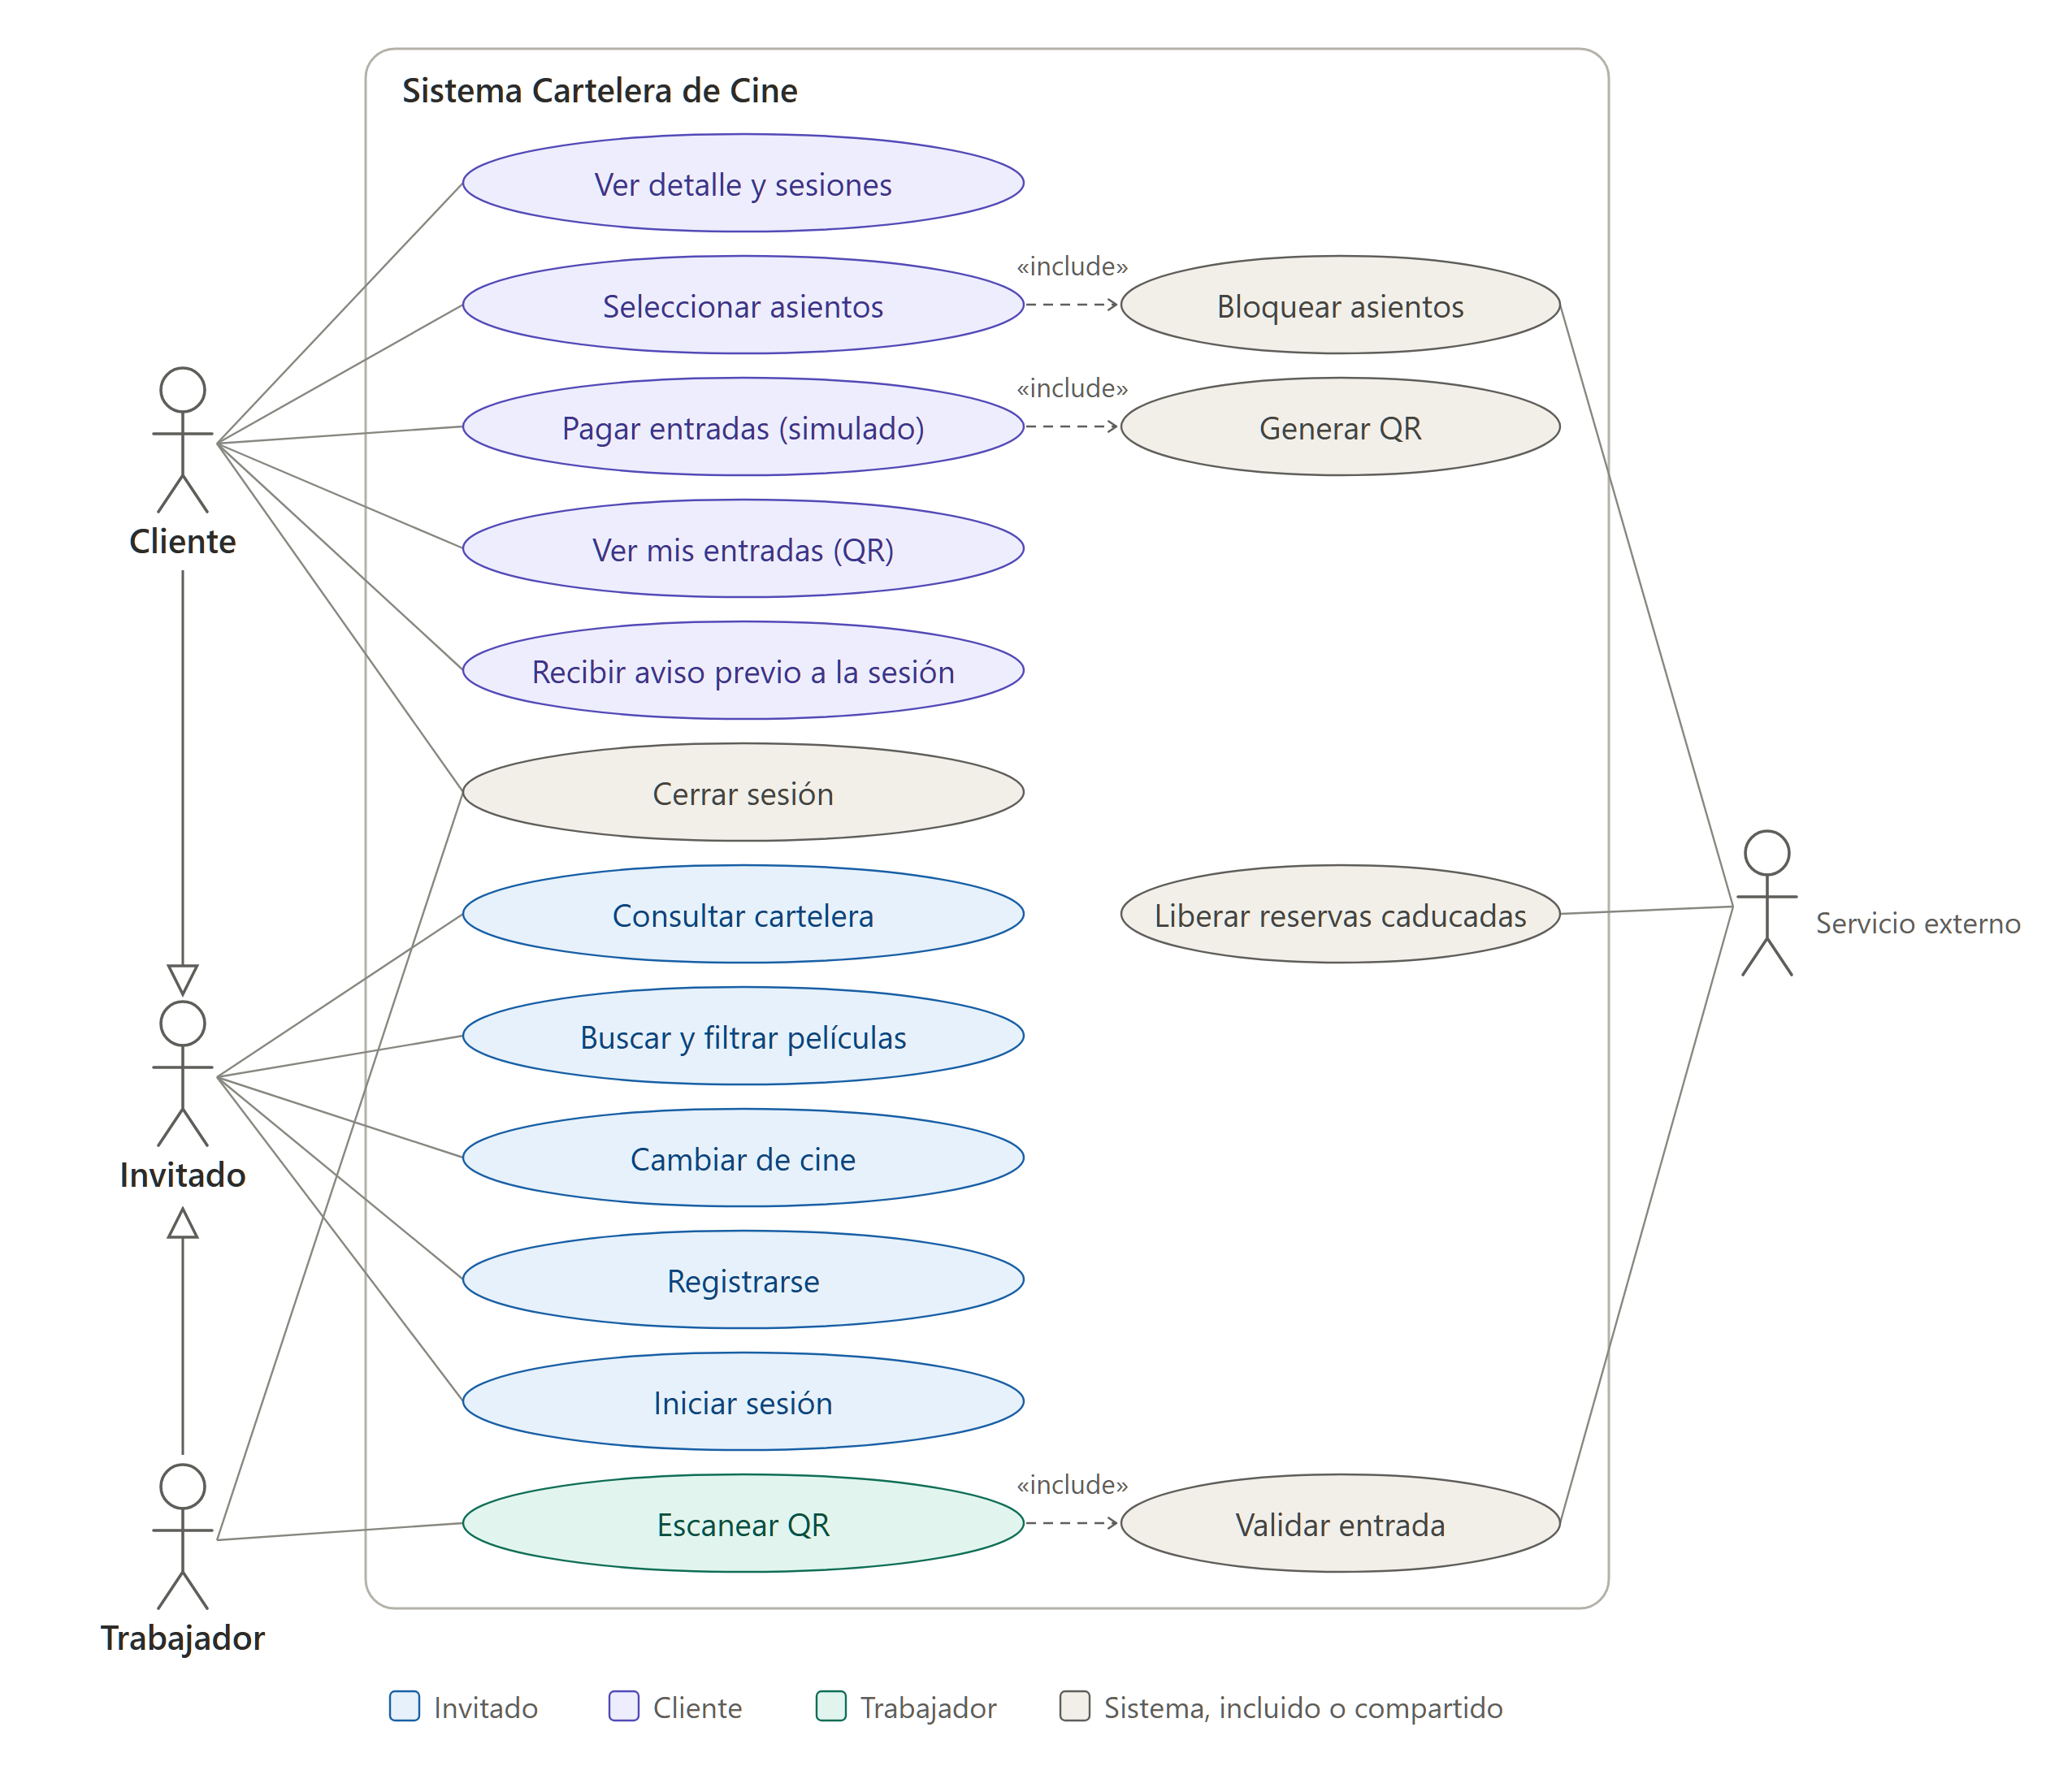
\includegraphics[width=0.9\textwidth]{casos-de-uso.png}
\caption{Diagrama de casos de uso (provisional).}
\label{fig:casos-uso}
\end{figure}

\newpage

\subsection{Especificación de Casos de Uso (CU)}
A continuación se detallan los dos casos de uso críticos de la aplicación, uno por cada rol, incluyendo su flujo principal y el tratamiento de situaciones de error (flujos alternativos).

\begin{longtable}{L{3.4cm} L{11.6cm}}
\toprule
\multicolumn{2}{l}{\textbf{CU-01: Compra de entradas}} \\
\midrule
\endfirsthead
\toprule
\multicolumn{2}{l}{\textbf{CU-01: Compra de entradas} (continuación)} \\
\midrule
\endhead
\bottomrule
\endfoot
\textbf{Requisitos asociados} & RF-06, RF-07, RF-08, RF-09, RF-11, RF-12, RNF-02, RNF-03 \\
\textbf{Actor principal} & ACT-02 (Cliente) \\
\textbf{Actores secundarios} & ACT-04 (Servicio externo) \\
\textbf{Precondiciones} & El usuario se encuentra en la cartelera y dispone de una cuenta de cliente. \\
\textbf{Flujo principal (Éxito)} &
1. El cliente, con la sesión iniciada, selecciona una película de la cartelera.\newline
2. La aplicación muestra el detalle de la película y sus sesiones disponibles.\newline
3. El cliente elige una sesión y la aplicación muestra el mapa de asientos de la sala.\newline
4. El cliente selecciona entre uno y ocho asientos libres y confirma.\newline
5. El sistema reserva los asientos a nombre del cliente durante 8 minutos y la aplicación muestra el tiempo restante.\newline
6. El cliente rellena el formulario de pago simulado y lo confirma antes de que caduque la reserva.\newline
7. El sistema genera una entrada con código QR por cada asiento.\newline
8. La aplicación programa el aviso una hora antes de la sesión y muestra la confirmación de la compra con acceso a «Mis entradas». \\
\textbf{Flujos alternativos (Errores)} &
\textbf{1a. Usuario sin sesión iniciada:} Al intentar abrir el detalle de una película, la aplicación lo dirige al inicio de sesión; una vez autenticado como cliente, el flujo continúa en el paso 2.\newline
\textbf{4a. Asiento no disponible:} Si otro usuario ha reservado antes alguno de los asientos, se informa «Algún asiento ya no está disponible» y se actualiza el mapa.\newline
\textbf{6a. Reserva caducada:} Si han pasado 8 minutos, se informa al cliente, los asientos se liberan y se vuelve al mapa de asientos.\newline
\textbf{6b. Fallo de red:} Se muestra un mensaje recuperable sin perder la selección; un reintento no genera entradas duplicadas.\newline
\textbf{8a. Menos de una hora para la sesión:} La compra se completa, pero no se programa el aviso. \\
\textbf{Postcondiciones} & Las entradas quedan almacenadas en la cuenta del cliente y visibles en «Mis entradas», los asientos quedan ocupados y, si procede, el aviso previo a la sesión queda programado. \\
\caption{Detalle del Caso de Uso CU-01.}\\
\end{longtable}

\begin{longtable}{L{3.4cm} L{11.6cm}}
\toprule
\multicolumn{2}{l}{\textbf{CU-02: Validación de una entrada mediante código QR}} \\
\midrule
\endfirsthead
\toprule
\multicolumn{2}{l}{\textbf{CU-02: Validación de una entrada mediante código QR} (continuación)} \\
\midrule
\endhead
\bottomrule
\endfoot
\textbf{Requisitos asociados} & RF-10, RNF-05, RNF-08 \\
\textbf{Actor principal} & ACT-03 (Trabajador) \\
\textbf{Actores secundarios} & ACT-04 (Servicio externo) \\
\textbf{Precondiciones} & El trabajador ha iniciado sesión correctamente, se encuentra en la pantalla de escaneo y ha concedido el permiso de cámara. \\
\textbf{Flujo principal (Éxito)} &
1. El trabajador apunta la cámara al código QR de la entrada que muestra el cliente.\newline
2. La aplicación lee el código, lo envía al sistema para validarlo y muestra que la validación está en curso.\newline
3. El sistema comprueba que la entrada existe y que no ha sido usada.\newline
4. El sistema marca la entrada como usada.\newline
5. La aplicación muestra el resultado en verde indicando la sala, la fila y el asiento. \\
\textbf{Flujos alternativos (Errores)} &
\textbf{1a. Permiso de cámara denegado:} Se explica el motivo y cómo concederlo desde los ajustes del dispositivo.\newline
\textbf{2a. Código no válido o falsificado:} Si el código no corresponde a ninguna entrada de la aplicación, se rechaza y se muestra en rojo el motivo.\newline
\textbf{2b. Fallo de red:} Se informa de que se necesita conexión para validar y se permite volver a escanear.\newline
\textbf{3a. Entrada ya usada:} Se muestra en rojo junto con la hora de su primer uso.\newline
\textbf{3b. Entrada de otra sesión:} Se rechaza y se muestra en rojo con el motivo. \\
\textbf{Postcondiciones} & La entrada válida queda marcada como usada y no puede volver a validarse. En los casos de rechazo, el estado de la entrada no se modifica. \\
\caption{Detalle del Caso de Uso CU-02.}\\
\end{longtable}

% ==========================================
% RESTO DE APARTADOS DE LA RÚBRICA
% ==========================================
\section{Diseño de la interfaz y experiencia de usuario}
En este apartado se describen las pantallas de la aplicación, su navegación según el rol del usuario y las decisiones de interacción adoptadas.

\subsection{Mapa de navegación}
La aplicación se abre siempre en la cartelera, que es la única pantalla accesible sin iniciar sesión. Desde ella, el usuario puede iniciar sesión o registrarse. Tras autenticarse, el flujo depende del rol: el cliente permanece en la cartelera y accede al resto del recorrido de compra, mientras que el trabajador es dirigido a la pantalla de escaneo de entradas.

\begin{table}[h!]
\centering
\begin{tabularx}{\textwidth}{L{3.6cm} L{3.4cm} Y}
\toprule
\textbf{Pantalla} & \textbf{Acceso} & \textbf{Descripción} \\
\midrule
Cartelera & Todos, incluido el invitado & Listado de películas del cine seleccionado, con búsqueda por título y género y selector de cine (RF-04, RF-05, RF-13). \\
Inicio de sesión y registro & Invitado & Autenticación y creación de cuenta; el código de trabajador es opcional (RF-01, RF-02). \\
Detalle de película & Cliente & Sinopsis, duración, género, clasificación por edad y sesiones (RF-06). \\
Mapa de asientos & Cliente & Selección de hasta 8 asientos de la sala con cuenta atrás de la reserva (RF-07). \\
Pago & Cliente & Formulario de pago simulado (RF-08). \\
Mis entradas & Cliente & Entradas compradas con su código QR (RF-09). \\
Perfil & Cliente y trabajador & Datos de la cuenta y cierre de sesión (RF-03). \\
Escaneo de entradas & Trabajador & Cámara para leer el código QR de la entrada (RF-10). \\
Resultado de validación & Trabajador & Entrada válida o rechazada, con sala, fila y asiento cuando es válida (RF-10). \\
\bottomrule
\end{tabularx}
\caption{Pantallas de la aplicación y rol con acceso.}
\end{table}

\subsection{Prototipos iniciales y evolución del diseño}
Las principales decisiones de interacción son las siguientes:
\begin{itemize}
    \item La cartelera es la pantalla de inicio para todos los usuarios, de modo que cualquier persona puede ver qué películas hay antes de decidirse a crear una cuenta.
    \item Los asientos se eligen sobre un mapa de la sala, que permite ver de un vistazo cuáles están libres, ocupados o seleccionados, y se muestra el tiempo restante de la reserva.
    \item El trabajador llega directamente a la pantalla de escaneo y el resultado de cada validación se muestra a pantalla completa, para poder leerlo rápidamente en la entrada de la sala.
\end{itemize}
\pendiente{Incluir los prototipos o bocetos iniciales, las capturas de las pantallas finales y los cambios realizados respecto al diseño inicial con su justificación.}

\subsection{Accesibilidad, legibilidad y adaptación a pantallas}
Se aplican los criterios del requisito RNF-09: contraste adecuado, tamaños táctiles mínimos de 48\,dp y descripciones de contenido en los elementos no textuales. Los estados no dependen únicamente del color: los asientos libres, ocupados y seleccionados se distinguen también por su forma o etiqueta, y el resultado de la validación incluye un texto (entrada válida o no válida) además del color verde o rojo. El código QR se muestra con un tamaño y contraste suficientes para ser leído por la cámara de otro dispositivo. Los diseños deben adaptarse a distintos tamaños de pantalla de móvil.

\section{Arquitectura de la aplicación}
\textit{Identificar y justificar la arquitectura adoptada. Incluir un diagrama de componentes o capas, sus responsabilidades y su comunicación, relacionándolo con la implementación real.}

\subsection{Justificación del patrón arquitectónico (MVVM / Clean Architecture)}
\subsection{Diagrama de capas y flujo de datos}

\pendiente{Completar cuando el equipo decida la arquitectura.}

\section{Gestión y persistencia de datos}
\textit{Explicar los datos y su modelo, relaciones y mecanismos de almacenamiento. Si existe base de datos, documentar su diseño. Si no es necesaria, justificarlo y describir la gestión del estado y de otros datos relevantes.}

\subsection{Modelo de datos y entidades}
\subsection{Estrategia de persistencia (Local / Remota)}

\pendiente{Completar cuando el equipo decida el modelo de datos y el almacenamiento.}

\section{Desarrollo e implementación}
\textit{Explicar la estructura de carpetas, ficheros y componentes principales, la gestión del estado, los patrones y las librerías. Describir la programación asíncrona utilizada (corrutinas en Kotlin). Documentar servicios, APIs o funciones del dispositivo y las decisiones técnicas relevantes.}

\subsection{Estructura de paquetes del proyecto}
\subsection{Gestión del estado reactivo y programación asíncrona (Corrutinas)}
\subsection{Servicios externos, librerías y recursos del dispositivo}

\pendiente{Completar cuando el equipo decida las tecnologías y durante el desarrollo.}

\section{Pruebas y validación}
\textit{Registrar casos de prueba con condiciones, acciones, resultado esperado y resultado obtenido. Identificar dispositivos o emuladores y versiones probadas, errores detectados y correcciones. Aportar evidencias de las funcionalidades principales y de errores relevantes; describir tests automatizados si los hay.}

\begin{longtable}{L{1.3cm} L{1.9cm} L{3.9cm} L{4.6cm} L{1.9cm}}
\caption{Registro de pruebas funcionales y de error.}\\
\toprule
\textbf{ID} & \textbf{Requisito} & \textbf{Condiciones y Acción} & \textbf{Resultado Esperado / Obtenido} & \textbf{Estado} \\
\midrule
\endfirsthead
\toprule
\textbf{ID} & \textbf{Requisito} & \textbf{Condiciones y Acción} & \textbf{Resultado Esperado / Obtenido} & \textbf{Estado} \\
\midrule
\endhead
\bottomrule
\endfoot

\textbf{CP-01} & RF-01 & Introducir un correo sin formato válido y pulsar registrarse. & \textbf{Esperado:} muestra un error de validación bajo el campo.\newline \textbf{Obtenido:} -- & Pendiente \\
\midrule
\textbf{CP-02} & RF-02 & Iniciar sesión con credenciales incorrectas. & \textbf{Esperado:} muestra «Correo o contraseña incorrectos».\newline \textbf{Obtenido:} -- & Pendiente \\
\midrule
\textbf{CP-03} & RF-04 & Abrir la aplicación sin iniciar sesión y seleccionar una película. & \textbf{Esperado:} se ve la cartelera y al seleccionar la película se dirige al inicio de sesión.\newline \textbf{Obtenido:} -- & Pendiente \\
\midrule
\textbf{CP-04} & RF-04, RNF-06 & Activar modo avión con la cartelera ya consultada y abrir la aplicación. & \textbf{Esperado:} muestra la cartelera guardada con un aviso, sin cerrar la aplicación.\newline \textbf{Obtenido:} -- & Pendiente \\
\midrule
\textbf{CP-05} & RF-07 & Dos clientes seleccionan el mismo asiento y el segundo confirma después. & \textbf{Esperado:} el segundo recibe «Algún asiento ya no está disponible» y el mapa se actualiza.\newline \textbf{Obtenido:} -- & Pendiente \\
\midrule
\textbf{CP-06} & RF-08, RF-11 & Reservar asientos y esperar más de 8 minutos antes de pagar. & \textbf{Esperado:} se informa de la caducidad, los asientos se liberan y se vuelve al mapa.\newline \textbf{Obtenido:} -- & Pendiente \\
\midrule
\textbf{CP-07} & RF-09 & Consultar las entradas sin conexión tras haberlas visto antes. & \textbf{Esperado:} se muestran las entradas con su código QR.\newline \textbf{Obtenido:} -- & Pendiente \\
\midrule
\textbf{CP-08} & RF-10 & Escanear con el trabajador el QR de una entrada válida. & \textbf{Esperado:} resultado en verde con sala, fila y asiento, y la entrada queda como usada.\newline \textbf{Obtenido:} -- & Pendiente \\
\midrule
\textbf{CP-09} & RF-10 & Escanear de nuevo el QR de una entrada ya usada. & \textbf{Esperado:} resultado en rojo con la hora del primer uso.\newline \textbf{Obtenido:} -- & Pendiente \\
\midrule
\textbf{CP-10} & RF-12 & Comprar una entrada para una sesión que empieza en más de una hora y esperar a la hora del aviso. & \textbf{Esperado:} una hora antes llega una notificación con el título de la película.\newline \textbf{Obtenido:} -- & Pendiente \\
\midrule
\textbf{CP-11} & RF-12 & Comprar una entrada para una sesión que empieza en menos de una hora. & \textbf{Esperado:} la compra se completa y no se programa ningún aviso.\newline \textbf{Obtenido:} -- & Pendiente \\
\midrule
\textbf{CP-12} & RF-13 & Abrir la aplicación denegando el permiso de ubicación y elegir un cine en el selector. & \textbf{Esperado:} la aplicación sigue funcionando, muestra el selector de cine y la cartelera se actualiza al cine elegido.\newline \textbf{Obtenido:} -- & Pendiente \\
\end{longtable}

\pendiente{Ejecutar las pruebas y completar el resultado obtenido y el estado de cada caso; indicar los dispositivos o emuladores y versiones de Android probados, los errores detectados y sus correcciones, adjuntar evidencias y describir los tests automatizados si los hay.}

\section{Proceso de desarrollo y gestión del proyecto}
\textit{Explicar etapas, organización del equipo, distribución de tareas y cambios de planificación. Incluir enlaces a issues, hitos, ramas y pull requests representativos y una síntesis de las aportaciones individuales.}

El código del proyecto se aloja en el repositorio de GitHub indicado en la portada.

\subsection{Organización del equipo y reparto de tareas}
\pendiente{Describir las etapas del proyecto, el reparto de tareas entre los integrantes del equipo, los cambios de planificación y la síntesis de las aportaciones individuales.}

\subsection{Flujo de trabajo en GitHub (Ramas, Issues, Hitos y Pull Requests)}
\pendiente{Describir el flujo de ramas utilizado e incluir enlaces a issues, hitos y pull requests representativos.}

\section{Uso de herramientas de IA generativa}
\textit{Declarar si se ha utilizado IA. En caso afirmativo, identificar herramientas, finalidad, partes del proyecto afectadas y ejemplos representativos de instrucciones y resultados. Explicar cómo se revisaron, adaptaron y comprobaron las aportaciones.}

\pendiente{Declarar el uso o no de herramientas de IA generativa y, en su caso, detallarlo según se indica arriba.}

\section{Conclusiones y trabajo futuro}
\textit{Valorar el cumplimiento de los objetivos con referencia a los resultados. Explicar dificultades, aprendizajes, limitaciones y mejoras pendientes, diferenciándolas de las funcionalidades entregadas.}

\pendiente{Redactar las conclusiones una vez finalizado el desarrollo y las pruebas.}

\section*{Fuentes consultadas y referencias}
\addcontentsline{toc}{section}{Fuentes consultadas y referencias}
\begin{itemize}
    \item Documentación oficial de Android Developers: \url{https://developer.android.com}
    \item Guía de arquitectura de aplicaciones Android: \url{https://developer.android.com/topic/architecture}
\end{itemize}

\end{document}
